\documentclass[10pt,mathserif]{beamer}

\usepackage{graphicx,amsmath,amssymb,tikz,psfrag,subfigure,bm}

\input defs.tex

%% formatting

\mode<presentation>
{
\usetheme{default}
}
\setbeamertemplate{navigation symbols}{}
\usecolortheme[rgb={0,0,0}]{structure}
\setbeamertemplate{itemize subitem}{--}
\setbeamertemplate{frametitle} {
	\begin{center}
	  {\large\bf \insertframetitle}
	\end{center}
}

\AtBeginSection[] 
{ 
	\begin{frame}<beamer> 
		\frametitle{Outline} 
		\tableofcontents[currentsection,currentsubsection] 
	\end{frame} 
} 

%% begin presentation

\title{\large \bfseries Variational Inference}

\author{Jiali Lin\\[3ex]
Virginia Tech}

\date{\today}

\begin{document}

\frame{
\thispagestyle{empty}
\titlepage
}

\section{Introduction}
\begin{frame}{Motivation}
\begin{itemize}
    \item \textbf{Variational inference:} deterministic approximate inference. 
    \item Pick an approximation $q(\bm{y})$ that are tractable family, and make this approximation close  to the true posterior, $p^*(\bm{y}) = p(\bm{y}|\mathcal{D})$.
    \item This reduces inference to an optimization problem.
    \item By approximating the objective, we can trade accuracy for speed.
    \item \textbf{Pros}:
    \begin{itemize}
        \item For small to medium problems, it is usually faster.
        \item It is deterministic.
        \item Is it easy to determine when to stop.
        \item It often provides a lower bound on the log likelihood.
    \end{itemize}
\end{itemize}    
\end{frame}

\section{Variational Inference}
\begin{frame}{Variational calculus}
Variational inference is based on variational calculus.
\bigskip
\begin{columns}
\column{0.5\textwidth}
\textbf{Standard Calculus} 
\begin{itemize}
    \item Functions $f:\bm{y}\rightarrow f(\bm{y})$.
    \item Derivatives $\frac{df}{d\bm{y}}$.
\end{itemize}
Example: maximize the likelihood expression $p(\bm{y}|\theta)$ w.r.t $\theta$.

\column{0.5\textwidth}
\textbf{Variational Calculus} 
\begin{itemize}
    \item Functionals $f:\bm{y}\rightarrow F(f)$.
    \item Derivatives $\frac{dF}{df}$.
\end{itemize}
Example: maximize the entropy $H[p]$ w.r.t a probability $p(\bm{y})$.
\end{columns}
\end{frame}

\begin{frame}{Variational calculus and the free energy}
By appropriate choice of $q(\bm{\theta})$, $F(q,\bm{y})$ becomes tractable to compute and maximize. Hence we have both an analytical approximation $q(\bm{\theta})$ for the posterior $p(\bm{\theta}|\bm{y})$ and a lower bound $F(q,\bm{y})$ for the evidence $\log p(\bm{y})$.
\bigskip
\begin{equation}\label{eq:1}
    \begin{split}
        \ln p(\bm{y})
        & = \ln \frac{p(\bm{y},\bm{\theta})}{p(\bm{\theta}|\bm{y})}\\
        & = \int q(\bm{\theta}) \ln \frac{p(\bm{y},\bm{\theta})}{p(\bm{\theta}|\bm{y})} d\bm{\theta} \ \ \ \xleftarrow{\ln p(\bm{y})\text{ does not depend on }\bm{\theta}}\\
        & = \int q(\bm{\theta}) \ln \frac{p(\bm{y},\bm{\theta})}{p(\bm{\theta}|\bm{y})} \frac{q(\bm{\theta})}{q(\bm{\theta})}d\bm{\theta} \\
        & = \int q(\bm{\theta}) (\ln \frac{q(\bm{\theta})}{p(\bm{\theta}|\bm{y})} + \ln \frac{p(\bm{y},\bm{\theta})}{q(\bm{\theta})})d\bm{\theta} \\        
        & = \int \underbrace{ q(\bm{\theta}) \ln \frac{q(\bm{\theta})}{p(\bm{\theta}|\bm{y})}d\bm{\theta}}_{\mbox{KL}[q||p] \text{ divergence}} +  \underbrace{\int q(\bm{\theta})\ln\frac{p(\bm{y},\bm{\theta})}{q(\bm{\theta})}d\bm{\theta}}_{F(q,\bm{y}) \text{ free energy }}
    \end{split}
\end{equation}
\end{frame}

\begin{frame}{Computing the free energy}
\begin{itemize}
    \item $\mbox{KL}[q||p]$ divergence is unknown and free energy $F(q,\bm{y})$ is easy to evaluate for a given $q$.
    \item Maximizing $F(q,\bm{y})$ is equivalent to minimizing $\mbox{KL}[q||p]$ and tightening $F(q,\bm{y})$ as a lower bound to ~\eqref{eq:1}.
\end{itemize}
\bigskip
We can decompose the free energy $F(q,\bm{y})$ as follows
\begin{equation}
    \begin{split}
        F(q,\bm{y}) 
        & = \int q(\bm{\theta})\ln\frac{p(\bm{y},\bm{\theta})}{q(\bm{\theta})}d\bm{\theta}\\
        & = \int q(\bm{\theta}) \ln p(\bm{y},\bm{\theta})d\bm{\theta} - \int q(\bm{\theta}) \ln q(\bm{\theta}) d\bm{\theta}\\
        & = \underbrace{<\ln p(\bm{y},\bm{\theta})>_q}_{\text{expected log-joint}} + \underbrace{H[q]}_{\text{Shannon entropy}}
    \end{split}
\end{equation}
\end{frame}

\begin{frame}{Forward or reverse KL?}
KL divergence is not symmetric in its arguments, minimizing $\mbox{KL}[q||p]$ wrt $q$ will give different behavior than minimizing $\mbox{KL}[q||p]$.
\begin{itemize}
    \item \textbf{Variational Bayes} minimize $\mbox{KL}[q(\bm{\theta})||p(\bm{\theta}|\bm{y})]$: $q(\bm{\theta})$ will tend to be zero where $p(\bm{\theta}|\bm{y})$ is zero. 
    \item \textbf{Expectation Propagation} minimize $\mbox{KL}[p(\bm{\theta}|\bm{y})||q(\bm{\theta})]$: $q(\bm{\theta})$ will tend to be nonzero where $p(\bm{\theta}|\bm{y})$ is nonzero.
\end{itemize}
    
\begin{figure}[h]
\centering     %%% not \center
\subfigure{\includegraphics[width=30mm]{{Figure10.2a}.pdf}}
\subfigure{\includegraphics[width=30mm]{{Figure10.2b}.pdf}}
\caption{Comparison of the two alternative forms for the Kullback-Leibler divergence.  (a) the Kullback-Leibler divergence $\mbox{KL}(q||p)$, and (b) the reverse Kullback-Leibler divergence $\mbox{KL}(p||q)$. Figure generated by \texttt{KLpqGauss}.}
\end{figure}
\end{frame}

\begin{frame}{Forward or reverse KL? (cont'd)}
\begin{figure}[h]
\centering     %%% not \center
\subfigure[]{\includegraphics[width=20mm]{{Figure10.3a}.pdf}}
\subfigure[]{\includegraphics[width=20mm]{{Figure10.3b}.pdf}}
\subfigure[]{\includegraphics[width=20mm]{{Figure10.3c}.pdf}}
\caption{Another comparison of the two alternative forms for the Kullback-Leibler divergence. (a) Averaging across modes may lead to poor predictive performance.  (b) (c) Variational Bayes may lead to local minimum. Figure generated by \texttt{KLfwdReverseMixGauss}.}
\end{figure}   
\end{frame}

\begin{frame}{Mean field approximation}
\textbf{Mean field approximation} assumes the posterior is a fully factorized approximation of the form
\begin{equation}
    q(\bm{\theta}) = \prod_i q_i(\bm{\theta}_i)
\end{equation}
\end{frame}

\begin{frame}{Derivation of the mean field update equations}
\begin{equation}\small
    \begin{split}
        F(q,\bm{y})
        & = \int q(\bm{\theta})\ln\frac{p(\bm{y},\bm{\theta})}{q(\bm{\theta})}d\bm{\theta}\\
        & = \int \prod_i q_i \times (\ln p(\bm{y},\bm{\theta}) - \sum_i \ln q_i)d\bm{\theta} \ \ \ \xleftarrow{\textbf{mean field assumption: }q(\bm{\theta}) = \prod_i q_i(\bm{\theta}_i)}\\
        & = \int q_j\prod_{\backslash j}q_i(\ln p(\bm{y},\bm{\theta}) - \ln q_i)d\bm{\theta} - \int q_j\prod_{\backslash j}q_i\sum_{\backslash j}\ln q_i d\bm{\theta}\\
        & = \int q_j (\underbrace{\int \prod_{\backslash j} q_i \ln p(\bm{y},\bm{\theta}) d\bm{\theta}_{\backslash_j}}_{<\ln p(\bm{y},\bm{\theta})>_{q\backslash j}}- \ln q_i)d\bm{\theta}_j - \int q_j \int\prod_{\backslash j}q_i \ln \prod_{\backslash j}q_i d\bm{\theta}_{\backslash_j}d\bm{\theta}_j\\
        & = \int q_j\ln\frac{\exp(<\ln p(\bm{y},\bm{\theta})>_{q\backslash j})}{q_j}d\bm{\theta}_j + c \ \ \ \xleftarrow{\exp(<\ln p(\bm{y},\bm{\theta})>_{q\backslash j})  = E_{\backslash j}[\ln p(\bm{y}, \bm{\theta})]}\\
        & = -\mbox{KL}[q_j||\exp(<\ln p(\bm{y},\bm{\theta})>_{q\backslash j})] + c
    \end{split}
\end{equation}
\end{frame}

\begin{frame}{Derivation of the mean field update equations(cont'd)}
Suppose the densities $q_{\backslash j} = q(\bm{\theta}_{\backslash j})$ are kept fixed. Then the approximate posterior $q(\bm{\theta}_j)$ that maximizes $F(q,\bm{y})$ is given by
\begin{equation}
    \begin{split}
        q_j^* 
        & = \max_{q_j}\ F(q,\bm{y})\\
        & = \frac{1}{Z}\exp(<\ln p(\bm{y},\bm{\theta})>_{q\backslash j}) 
    \end{split}
\end{equation}

Therefore:
\begin{equation}
    \ln q_j^* = <\ln p(\bm{y},\bm{\theta})>_{q\backslash j} - \ln Z
\end{equation}

where $Z = \int <\ln p(\bm{y},\bm{\theta})>_{q\backslash j} d \bm{\theta}_j$. \bigskip
    
This implies a straightforward algorithm for variational inference: 
\begin{enumerate}
    \item Initialize all approximate posteriors $q(\bm{\theta}_i)$, e.g., by setting them to their priors.
    \item Cycle over the parameters, revising each given the current estimates of the others.
    \item Loop until convergence.
\end{enumerate}
\end{frame}

\section{Variational Bayes}
\begin{frame}{Introduction}
\begin{itemize}
    \item So far we are inferring latent variables $\bm{z}_i$ assuming the parameters $\bm{\theta}$ of the model are known.
    \item Now infer the parameters themselves.
    \item Mean field approximation
    \begin{equation}
        p(\bm{\theta}|\mathcal{D}) \approx \prod_i q_i(\bm{\theta}_i)
    \end{equation}
    \item This is \textbf{variational Bayes}  or \textbf{VB}.
    \item If we want to infer both latent variables and parameters, then 
    \begin{equation}
        p(\bm{\theta}, \bm{z}_{1:N}|\mathcal{D}) \approx q (\bm{\theta})\prod_i q_i(\bm{z}_i)
    \end{equation}
\end{itemize}
\end{frame}

\begin{frame}{Example: VB for a univariate Gaussian}
\begin{itemize}
    \item Assuming there are no latent variables.
    \item Consider applying VB to infer the posterior over the parameters for a 1d Gaussian, $p(\mu, \lambda|\mathcal{D})$, where $\lambda = 1/\sigma^2$ is the precision.
    \item For convenience, we will use a conjugate prior of the form. 
    \begin{equation}
        \begin{split}
            p(\mu, \lambda) & = p(\mu|\lambda)p(\lambda)\\
                            & = N (\mu|\mu_0,(\kappa_0\lambda) ^{-1})\mbox{Ga}(\lambda|a_0, b_0)  
        \end{split}
    \end{equation}
    \item Consider a factorized variational approximation
    \begin{equation}
        q(\mu, \lambda) = q_\mu(\mu)q_\lambda(\lambda)
    \end{equation}
\end{itemize}
\end{frame}


\begin{frame}{Target distribution}
The unnormalized log posterior has the form
\begin{equation}
    \begin{split}
        \log\widetilde{p}(\mu, \lambda) 
        & = \log p(\mu, \lambda, D) = \log p(D|\mu, \lambda) + \log p(\mu|\lambda) + \log p(\lambda) \\
        & = \frac{N}{2} \log \lambda - \frac{\lambda}{2}\sum_{i=1}^N (x_i - \mu)^2 - \frac{1}{2}\log(\kappa_0\lambda)\\
        & + \frac{\kappa_0\lambda}{2}  (\mu - \mu_0)^2 + (a_0 - 1)\log\lambda - b_0\lambda + \mbox{const}
    \end{split}
\end{equation}
\end{frame}

\begin{frame}{Updating $q_\mu(\mu)$ (fix $q_\lambda(\lambda)$)}
The optimal form for $q_\mu(\mu)$ is obtained by averaging over $\lambda$
\begin{equation}
    \begin{split}
        \log q_\mu(\mu) 
        & = E_{q_\lambda} [\log p(D|\mu, \lambda) + \log p(\mu|\lambda)] + \mbox{const}\\
        & = -\frac{E_{q_\lambda} [\lambda]}{2} \{\kappa_0(\mu - \mu_0)^2 + \sum_{i=1}^2 (x_i - \mu)^2 \} + \mbox{const}
    \end{split}
\end{equation}

By completing the square one can show that $q_\mu(\mu) = N (\mu|\mu_N , \kappa_N^{-1} )$, where 
\begin{equation}
    \begin{split}
        \mu_N & = \frac{\kappa_0\mu_0 + N\bar{x}}{\kappa_0 + N}\\
        \kappa_N & = (\kappa_0 + N)E_{q_\lambda} [\lambda]
    \end{split}
\end{equation}
 At this stage we don't know what $q_\lambda(\lambda)$ is, and hence we cannot compute $E [\lambda]$, but we will derive this below.
\end{frame}

\begin{frame}{Updating $q_\lambda(\lambda)$ (fix $q_\mu(\mu)$)}
The optimal form for $q_\lambda(\lambda)$ is given by 
\begin{equation}
    \begin{split}
        \log q_\lambda(\lambda) 
        & = E_{q_\mu} [\log p(D|\mu, \lambda) + \log p(\mu|\lambda) + \log p(\lambda)] + \mbox{const} \\
        & = (a_0 - 1) \log \lambda - b_0\lambda + \frac{1}{2}\log \lambda + \frac{N}{2} \log \lambda \\
        & -\frac{\lambda }{2} E_{q_\mu} [\kappa_0(\mu - \mu_0)^2 +\sum_{i=1}^N (x_i - \mu)^2 ] + \mbox{const}
    \end{split}
\end{equation}

We recognize this as the log of a Gamma distribution, hence $q_\lambda(\lambda) = \mbox{Ga}(\lambda|a_N , b_N )$, where
\begin{equation}\small
    \begin{split}
        a_N & = a_0 + \frac{N + 1}{2}\\
        b_N & = b_0 + \frac{1}{2} E_{q_\mu} [\kappa_0(\mu - \mu_0)^ 2 +\sum_{i=1}^N (x_i - \mu)^2 ] 
    \end{split}
\end{equation}
\end{frame}

\begin{frame}{Computing the expectations}
Since $q(\mu) = N (\mu|\mu_N , \kappa_N^{-1 })$, we have 
\begin{equation}\small
    \begin{split}
        E_{q(\mu)} [\mu]   & = \mu_N \\
        E_{q(\mu)} [\mu^2] & = \frac{1}{\kappa_N}+ \mu_N^2
    \end{split}
\end{equation}

Since $q(\lambda) = \mbox{Ga}(\lambda|a_N , b_N )$, we have
\begin{equation}
    E_q(\lambda) [\lambda] = \frac{a_N}{b_N}  
\end{equation}

Explicit forms for the update equations for $q(\mu)$ we have 
\begin{equation}\small
    \begin{split}
        \mu_N  & = \frac{\kappa_0\mu_0 + N\bar{x}}{\kappa_0 + N} \xleftarrow{\text{fixed!}}\\
        \kappa_N & = (\kappa_0 + N) \frac{a_N}{b_N}
    \end{split}
\end{equation}

and for $q(\lambda)$ we have 
\begin{equation}\small
    \begin{split}
        a_N & = a_0 + \frac{N + 1}{2} \xleftarrow{\text{fixed!}}\\
        b_N & = b_0 + \kappa_0(E [\mu^2] + \mu_0^2 - 2E[\mu] \mu_0) + \frac{1}{2} \sum_{i=1}^N (x_i^2 + E[\mu^2]-2E [\mu]- x_i)
    \end{split}
\end{equation}
\end{frame}

\begin{frame}{Illustration}
In the Figure, the green contours represent the exact posterior, which is Gaussian-Gamma. The dotted red contours represent the variational approximation over several iterations.

\begin{figure}[h]
\centering
\subfigure[]{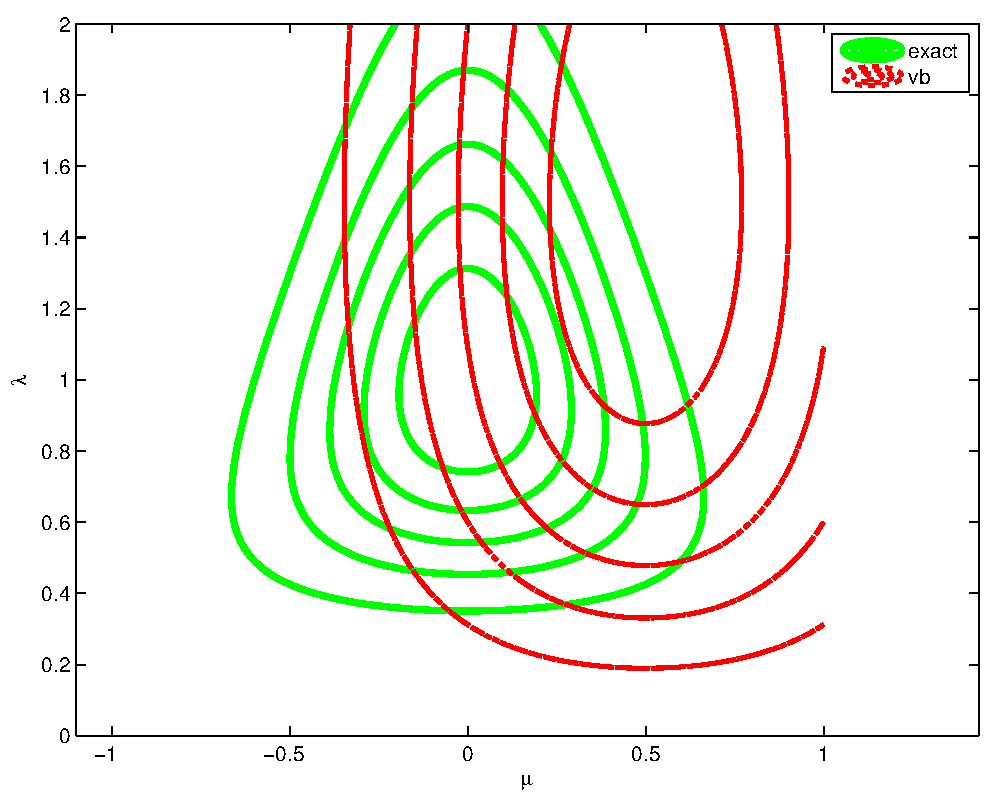
\includegraphics[width=20mm]{unigaussVbDemo1}}
\subfigure[]{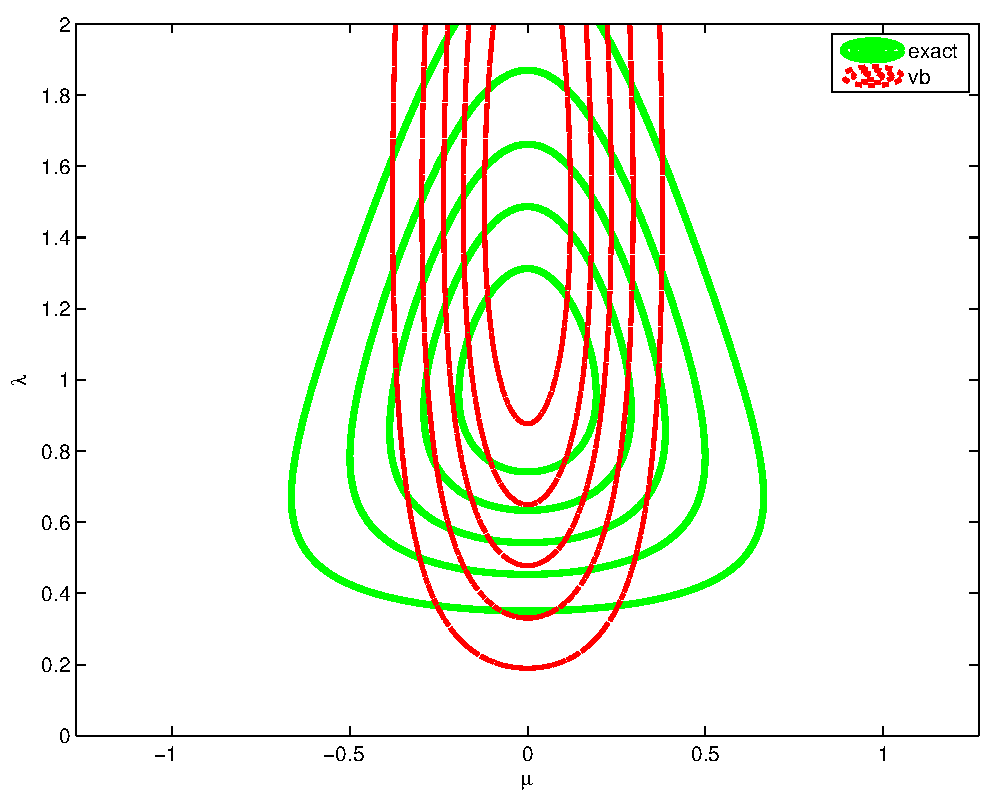
\includegraphics[width=20mm]{unigaussVbDemo2}}\\
\subfigure[]{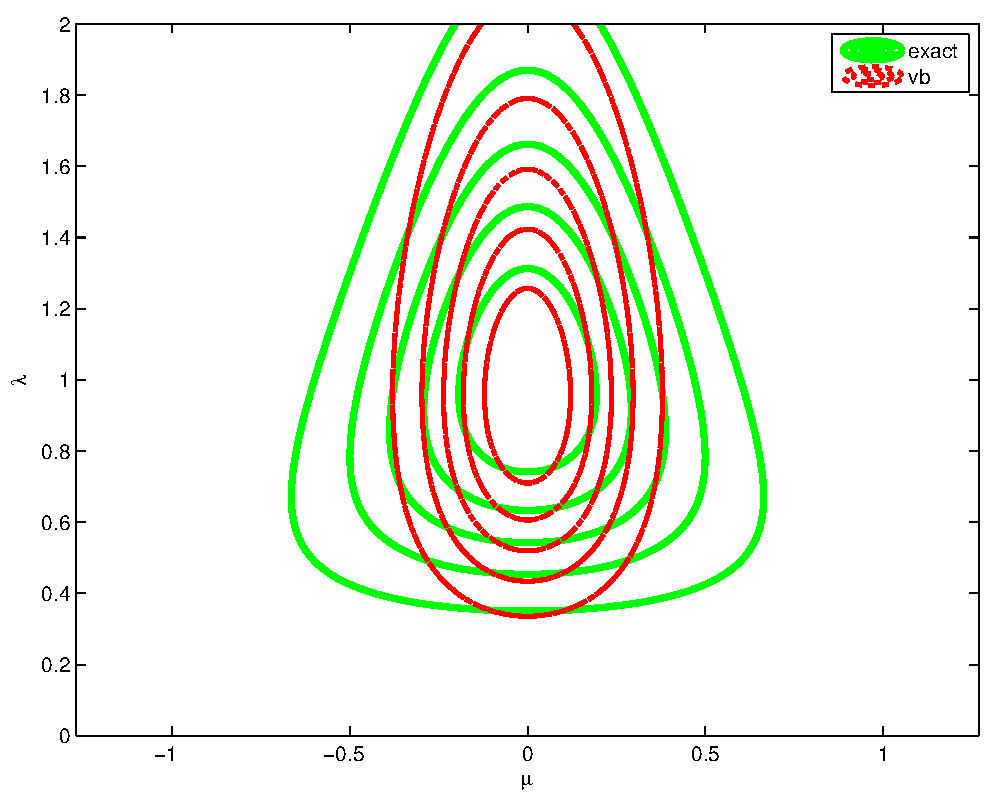
\includegraphics[width=20mm]{unigaussVbDemo3}}
\subfigure[]{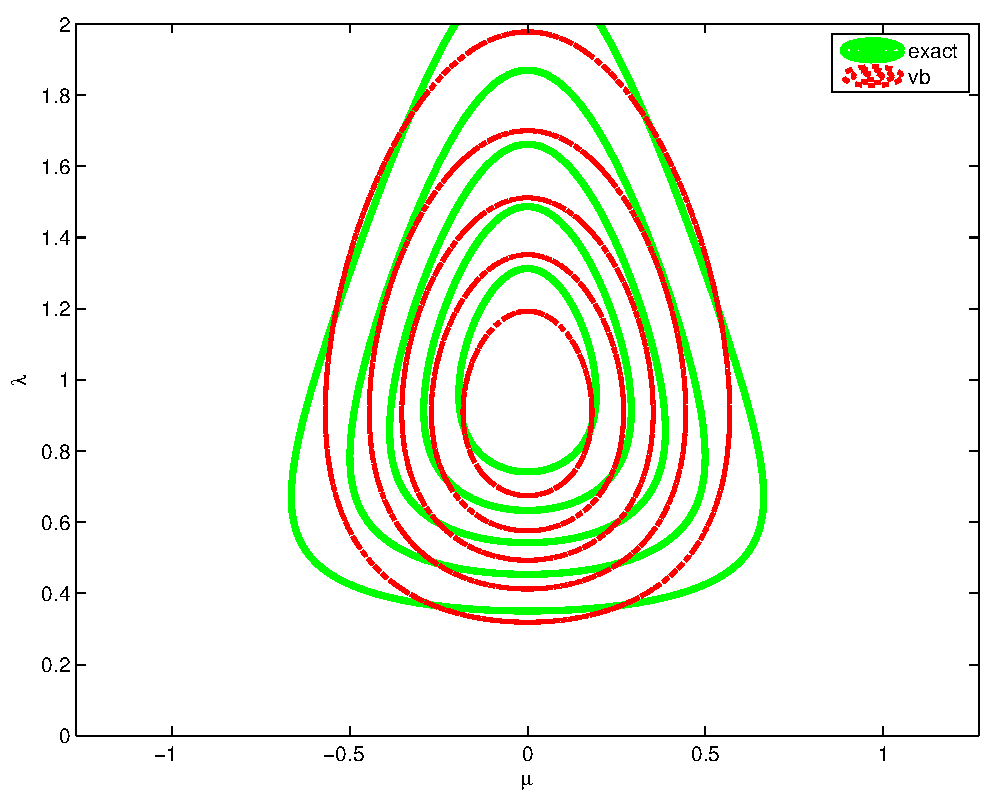
\includegraphics[width=20mm]{unigaussVbDemo4}}
\caption{Factored variational approximation (red) to the Gaussian-Gamma distribution (green). (a) Initial guess. (b) After updating $q_\mu$. (c) After updating $q_\lambda$. (d) At convergence (after 5 iterations). Based on 10.4 of (Bishop 2006b). Figure generated by \texttt{UnigaussVbDemo}.}
\end{figure}
\end{frame}        
        
\section{Variational Bayes EM}
\begin{frame}{Introduction}
\begin{itemize}
    \item Now consider latent variable models of the form $\bm{z}_i \rightarrow \bm{x}_i \leftarrow \bm{\theta}$.
    \item In EM, $\bm{\theta}$ are informed by all $N$ data cases, whereas $\bm{z}_i$ is only informed by $\bm{x}_i$.
    \item \textbf{Variational Bayes EM} or \textbf{VBEM}: model uncertainty in $\bm{\theta}$ and $\bm{z}_i$.
    \item Computational cost is essentially the same as EM.
    \item \textbf{Same idea}
    \begin{equation}
        p(\bm{\theta}, \bm{z}_{1:N}|\mathcal{D}) \approx q (\bm{\theta})\prod_i q_i(\bm{z}_i)
    \end{equation}
    \item \textbf{Pros:} marginalizing out the parameters, we can compute a lower bound on the marginal likelihood (useful for model selection).
\end{itemize} 
\end{frame}

\begin{frame}{The variational posterior}
\begin{itemize}
    \item The conditional distribution of $\bm{Z}$, given the mixing coefficients $\bm{\pi}$:
    \begin{equation}\small\label{eq:21}
        p(\bm{Z}|\bm{\pi}) = \prod_{n=1}^N \prod_{k=1}^K \pi_k^{z_{nk}}
    \end{equation}
    \item The likelihood:
    \begin{equation}\small\label{eq:22}
        p(\bm{X}|\bm{Z},\bm{\mu}, \bm{\bm{\Lambda}}) = \prod_{n=1}^N \prod_{k=1}^K N(\bm{X}_n|\bm{\mu}_k,\bm{\Sigma}_k^{-1})^{z_{nk}}
    \end{equation}
    \item Priors over the parameters $\bm{\mu}, \bm{\Sigma}$ and $\bm{\pi}$
    \begin{itemize}
        \item Pick a Dirichlet distribution over the mixing coefficients $\bm{\pi}$
    \begin{equation}\small
        p(\bm{\pi}) = \text{Dir}(\bm{\pi}|\bm{\alpha}_0) = C(\bm{\alpha}_0)\prod_{k=1}^K \bm{\pi}_k^{\alpha_0 - 1}
    \end{equation}
        \item Pick an independent Gaussian-Wishart prior for the mean and precision of each Gaussian component
    \begin{equation}\small
        \begin{split}
            p(\bm{\mu}, \bm{\Lambda}) & = p(\bm{\mu}|\bm{\Lambda})p(\bm{\Lambda})\\
            & = \prod_{k=1}^K N(\bm{\mu}_k|\bm{m}_0,(\beta_0\bm{\Lambda}_k)^{-1})W(\bm{\Lambda}_k|\bm{W}_0,\nu_0)
        \end{split}
    \end{equation}
    \end{itemize}
\end{itemize}
\end{frame}

\begin{frame}{The variational posterior (cont'd)}
\begin{itemize}
    \item The joint distribution of all of the random variables
    \begin{equation}
        p(\bm{X}, \bm{Z}, \bm{\pi}, \bm{\mu}, \bm{\Lambda}) = p(\bm{X}|\bm{Z}, \bm{\mu}, \bm{\Lambda})p(\bm{Z}|\bm{\pi})p(\bm{\pi})p(\bm{\mu}|\bm{\Lambda})p(\bm{\Lambda})
    \end{equation}
    \item Consider a variational distribution
    \begin{equation}
        q(\bm{Z}, \bm{\pi}, \bm{\mu}, \bm{\Lambda}) = q(\bm{Z})q(\bm{\pi}, \bm{\mu}, \bm{\Lambda})
    \end{equation}
    \textbf{Factors $q(\bm{Z})$ and $q(\bm{\pi}, \bm{\mu}, \bm{\Lambda})$ will be determined automatically by optimization of the variational distribution}.
\end{itemize}

\bigskip
\begin{figure}[h]
\centering
\includegraphics[width=0.3\textwidth]{{Figure10.5}.pdf}
\caption{DAG of the Bayesian mixture of Gaussians model.}
\end{figure}
\end{frame}

\begin{frame}{Derivation of $q(z)$ (variational E step)}
Update for the factor $q(\bm{Z})$
\begin{equation}\small
    \begin{split}
        \ln q^*(\bm{Z}) & =  E_{\bm{\pi}, \bm{\mu}, \bm{\Lambda}}[\ln p(\bm{X},\bm{Z},\bm{\pi}, \bm{\mu}, \bm{\Lambda})] + \text{const}\\
        & = E_{\bm{\pi}}[\ln p(\bm{Z}|\bm{\pi})]+E_{\bm{\mu}, \bm{\Lambda}}[\ln p(\bm{X}|\bm{Z},\bm{\mu}, \bm{\Lambda})] + \text{const}\\
        & = \sum_{n=1}^N\sum_{k=1}^K z_{nk}\ln \rho_{nk} + \text{const}
    \end{split}
\end{equation}

where we have defined
\begin{equation}\small
\ln\rho_{nk} = E[\ln\pi_k]+ \frac{1}{2}E[\ln|\bm{\Lambda}_k|]- \frac{D}{2} \ln(2\pi) - \frac{1}{2}E_{\bm{\mu}_k,\bm{\Lambda}_k} (\bm{x}_n - \bm{\mu}_k)^T \bm{\Lambda}_k (\bm{x}_n - \bm{\mu}_k)]
\end{equation}

Taking the exponential of both sides, we obtain
\begin{equation}\small
    q^*(\bm{Z}) \propto \prod_{n=1}^N\prod_{k=1}^K\rho_{nk}^{z_{nk}}
\end{equation}

\end{frame}

\begin{frame}{Derivation of $q(z)$ (variational E step) (cont'd)}
The factor $q(\bm{Z})$
\begin{itemize}
    \item Requires be normalized
    \begin{equation}\small
        q^*(\bm{Z}) \propto \prod_{n=1}^N\prod_{k=1}^K r_{nk}^{z_{nk}}    
    \end{equation}
    where $r_{nk} = \frac{\rho_{nk}}{\sum_{j=1}^K \rho_{nj}}$.
    \item Takes the same functional form as the prior $p(\bm{Z}|\bm{\pi})$.
    \item The discrete distribution $q(\bm{Z})$ have $E[z_{nk}] = r_{nk}$.
    \item The quantities $r_{nk}$ are playing the role of responsibilities.
    \item Three statistics evaluated with respect to the responsibilities
    \begin{equation}\small
        \begin{split}
            N_k & = \sum_{n=1}^N r_{nk}\\
            \bar{\bm{x}}_k & = \frac{1}{N_k}\sum_{n=1}^N r_{nk}\bm{x}_n\\
            \bm{S}_k & = \frac{1}{N_k}\sum_{n=1}^N r_{nk}(\bm{x}_n - \bar{\bm{x}}_k)(\bm{x}_n - \bar{\bm{x}}_k)^T
        \end{split}
    \end{equation}
\end{itemize}
\end{frame}

\begin{frame}{Derivation of $q(\theta)$ (variational M step)}
Consider the factor $q(\bm{\pi}, \bm{\mu}, \bm{\Lambda})$ in the variational posterior distribution
\begin{equation}\small\label{eq:32}
    \begin{split}
        \ln q(\bm{\pi}, \bm{\mu}, \bm{\Lambda}) & = \ln p(\bm{\pi}) + \sum_{k=1}^K\ln p(\bm{\mu}, \bm{\Lambda}) + E_{\bm{Z}}[\ln p(\bm{Z}|\bm{\pi})] \\ 
        & + \sum_{n=1}^N \sum_{k=1}^K E[z_{nk}] \ln N(\bm{x}_n|\bm{\mu}_k, \bm{\Lambda}_k^{-1}) + \text{const}
    \end{split}
\end{equation}

This decomposes into terms involving only $\bm{\pi}$ with only $\bm{\mu}$ and $\bm{\Lambda}$. Thus
\begin{equation}\small\label{eq:33}
    q(\bm{\pi}, \bm{\mu}, \bm{\Lambda}) = q(\bm{\pi}) \prod_{k=1}^K q(\bm{\mu}_k,\bm{\Lambda}_k)
\end{equation}

Identifying the terms on the right-hand side of~\eqref{eq:32} that depend on $\bm{\pi}$
\begin{equation}\small
    \ln q^* (\bm{\pi}) = (\alpha_0 -1) \sum_{k=1}^K \ln \bm{\pi}_k + \sum_{k=1}^K\sum_{n=1}^N r_{nk}\ln\bm{\pi}_k +\text{const} 
\end{equation}

Taking the exponential of both sides, $q^* (\bm{\pi})$ is a Dirichlet distribution
\begin{equation}
    q^*(\bm{\pi}) = \text{Dir}(\bm{\pi}|\alpha)
\end{equation}

where $\alpha$ has components $\alpha_k$ given by $\alpha_k = \alpha_0 + N_k$.
\end{frame}

\begin{frame}{Derivation of $q(\theta)$ (variational M step) (cont'd)}
Recall: $q (\bm{\mu}_k,\bm{\Lambda}_k) = q (\bm{\mu}_k|\bm{\Lambda}_k)q (\bm{\Lambda}_k)$. Thus
\begin{equation}\small
    q(\bm{\mu}_k, \bm{\Lambda}_k) = N (\bm{\mu}_k|\bm{m}_k, (\beta_k\bm{\Lambda}_k)^{-1}) W(\bm{\Lambda}_k|\bm{W}_k, \nu_k)
\end{equation}

where we defined
\begin{equation}\small~\label{eq:37}
    \begin{split}
        \beta_k & = \beta_0+N_k\\
        \bm{m}_k & = \frac{1}{\beta_k} (\beta_0\bm{m}_0 +N_k \bar{\bm{x}}_k)\\
        \bm{W}_k^{-1} & = \bm{W}_0^{-1}+N_k S_k + \frac{\beta_0 N_k}{\beta_0 + N_k}(\bar{\bm{x}}_k - \bm{m}_0)(\bar{\bm{x}}_k - \bm{m}_0)^T\\
        \nu_k & = \nu_0+N_k
    \end{split}
\end{equation}

Expectations of the variational distributions of the parameters
\begin{equation}\label{eq:38}\scriptsize
    \begin{split}
        E_{\bm{\mu}_k,\bm{\Lambda}_k} [(\bm{x}_n - \bm{\mu}_k)^T\bm{\Lambda}_k(\bm{x}_n - \bm{\mu}_k) & =  D\beta_k^{-1} + \nu_k(\bm{x}_n - \bm{m}_k)^T \bm{W}_k(\bm{x}_n - \bm{m}_k)] \\
        \ln\tilde{\bm{\Lambda}}_k & = E[\ln |\bm{\Lambda}_k|] = \sum_{i=1}^D \psi (\frac{\nu_k + 1 -i}{2}) + D\ln2 + \ln|\bm{W}_k|\\
        \ln\tilde{\bm{\pi}}_k & = E[\ln\bm{\pi}_k] = \psi(\alpha_k) - \psi(\hat{\alpha})
    \end{split}
\end{equation}

where we define $\tilde{\bm{\Lambda}}_k$ and $\tilde{\bm{\pi}}_k$, $\psi(.)$ is a the diagmma function, $\hat{\alpha} = \sum_k\alpha_k$.
\end{frame}

\begin{frame}{Derivation of $q(\theta)$ (variational M step) (cont'd)}
If we substitute~\eqref{eq:38} into $r_{nk} = \frac{\rho_{nk}}{\sum_{j=1}^K \rho_{nj}}$
\begin{equation}
    r_{nk} \propto \tilde{\bm{\pi}}_k \tilde{\bm{\Lambda}}_k^{1/2}\exp\{-\frac{D}{2\beta_k}-\frac{\nu_k}{2}(\bm{x}_n - \bm{m}_k)^T \bm{W}_k (\bm{x}_n - \bm{m}_k) \}
\end{equation}

Notice the similarity to the responsibilities in maximum likelihood EM
\begin{equation}
    r_{nk} \propto \bm{\pi}_k |\bm{\Lambda}_k|^{1/2}\exp\{-\frac{1}{2}(\bm{x}_n - \bm{\mu}_k)^T \bm{\Lambda}_k (\bm{x}_n - \bm{\mu}_k) \}
\end{equation}
\end{frame}

\begin{frame}{Lower bound on the marginal likelihood}
In VB, we are maximizing a lower bound on the log marginal likelihood. Why?
\begin{itemize}
    \item To assess convergence of the algorithm. 
    \item To assess the correctness of one's code: as with EM, if the bound does not increase monotonically, there must be a bug.
    \item To approximateto the marginal likelihood, which can be used for \textbf{Bayesian model selection}.
\end{itemize}

The algorithm is trying to maximize the following lower bound (i.e. $F(q,y)$ free energy)
\begin{equation}
    L = \sum_{\bm{Z}}\int\int\int q(\bm{Z},\bm{\pi},\bm{\mu},\bm{\Lambda})\ln\{\frac{p(\bm{X},\bm{Z},\bm{\pi},\bm{\mu},\bm{\Lambda})}{(Z,\bm{\pi},\bm{\mu},\bm{\Lambda})}\}d\bm{\pi}\ d\bm{\mu}\ d\bm{\Lambda} \leq \ln p(\bm{X})    
\end{equation}

This quantity increases monotonically with each iteration, in Figure. (Exercise)
\end{frame}

\begin{frame}{Posterior predictive distribution}
The predictive density is then given by
\begin{equation}
    p(\bm{x}^*|\bm{X}) = \sum_{\bm{z}^*}\int\int\int p(\bm{x}^*|\bm{z}^*,\bm{\mu},\bm{\Lambda}) p(\bm{z}^*|\bm{\pi})p(\bm{\pi},\bm{\mu},\bm{\Lambda}|\bm{X})d\bm{\pi}\ d\bm{\mu}\ d\bm{\Lambda}
\end{equation}

Using~\eqref{eq:21} and~\eqref{eq:22} we can first perform the summation over $\bm{z}^*$
\begin{equation}
    p(\bm{x}^*|\bm{X}) = \sum_{k=1}^K\int\int\int \pi_k N(\bm{x}^*|\bm{\mu}_k,\bm{\Lambda}_k^{-1})p(\bm{\pi},\bm{\mu},\bm{\Lambda}|\bm{X})d\bm{\pi}\ d\bm{\mu}\ d\bm{\Lambda}
\end{equation}

Because the remaining integrations are intractable, we approximate the predictive density with  $q(\bm{\pi})q(\bm{\mu},\bm{\Lambda})$
\begin{equation}
    p(\bm{x}^*|\bm{X}) = \sum_{k=1}^K\int\int\int \pi_k N(\bm{x}^*|\bm{\mu}_k,\bm{\Lambda}_k^{-1})q(\bm{\pi})q(\bm{\mu},\bm{\Lambda})d\bm{\pi}\ d\bm{\mu}\ d\Lambda
\end{equation}

where we have made use of the factorization~\eqref{eq:33}. 
\end{frame}

\begin{frame}{Posterior predictive distribution (cont'd)}
The remaining integrations can now be evaluated analytically giving a mixture of Student's t-distributions
\begin{equation}~\label{eq:45}
    p(\bm{x}^*|\bm{X}) = \frac{1}{\hat{\alpha}}\sum_{k=1}^K\alpha_k\text{St}(\bm{x}^*|\bm{m}_k,\bm{L}_k,\nu + 1 -D)
\end{equation}

in which the $k^{\text{th}}$ component has mean $\bm{m}_k$, and the precision is
\begin{equation}
    \bm{L}_k = \frac{(\nu_k +1 -D)\beta_k}{1+\beta_k}\bm{W}_k
\end{equation}
in which $\nu_k$ is given by~\eqref{eq:37}. When the size $
N$ of the data set is large the predictive distribution~\eqref{eq:45} reduces to a mixture of Gaussians.
\end{frame}

\end{document}
